\documentclass[journal]{IEEEtran}

\usepackage[pdftex]{graphicx}
\graphicspath{{img/}}
\usepackage{cite}
\usepackage{amsmath}
\DeclareMathOperator*{\argmin}{arg\,min}
\usepackage{amssymb}
\usepackage{mathtools}
\usepackage{booktabs,siunitx}
\usepackage{threeparttable}
%\usepackage{subcaption}
\usepackage{multirow}
\usepackage[caption=false,font=footnotesize,labelfont=sf,textfont=sf]{subfig}

%\usepackage{endfloat}

% TODO: remove
	\usepackage{xcolor}
	\newcommand\TODO[1]{\textcolor{red}{TODO: #1}}
	\newcommand\FIXME[1]{\textcolor{blue}{FIXME: #1}}

\begin{document}
\title{Automatic Brain Tissue Segmentation in MRI using Supervised Machine Learning}

\author{Michael~Rebsamen\textsuperscript{*},
        Jan~Riedo\textsuperscript{*},
        Michael~Mueller\textsuperscript{*}
\thanks{\textsuperscript{*}All authors contributed equally. Biomedical~Engineering, University~of~Bern. Authors~e-mail: michael.mueller4@students.unibe.ch, jan.riedo@students.unibe.ch, michael.rebsamen@students.unibe.ch}}
\markboth{Biomedical Engineering, Medical Image Analysis Lab, \today}
{}%2nd title, required for the primary to appear
% The only time the second header will appear is for the odd numbered pages
% after the title page when using the twoside option.
\maketitle

\begin{abstract}
Machine learning (ML), white matter (WM), grey matter (GM), cerebrospinal fluid (CSF), background (BG)
\end{abstract}
\begin{IEEEkeywords}
MRI, Segmentation, Machine Learning, DF, kNN, SVM
\end{IEEEkeywords}


\section{Introduction}\label{s.introduction}
Segmentation of brain tissues from magnetic resonance images (MRI) has many clinical applications. Clinicians gain useful information from a separation of tissue into its three main anatomical types: white matter (WM), grey matter (GM), and cerebrospinal fluid (CSF). Voxel-based morphometric measures have been used to investigate brain disorders like Alzheimer’s disease~\cite{busatto2003voxel}, Parkinson's disease~\cite{price2004voxel} or temporal lobe epilepsy~\cite{rummel2017personalized}. However, manual segmentation of MRI is a labour-intensive task requiring expert skills. Fully automatic approaches for brain tissue segmentation are therefore a topic of active research. A good algorithm classifies the tissue types with high accuracy across a variety of images from different patients. Such a classification is a typical task for machine learning. These algorithms tend to perform well given enough training data during the learning phase. The availability of ground-truth data in sufficient quantity and quality for supervised learning is a particular challenge when working with medical images due to privacy concerns and the costs for manual segmentation. Optimization of the learning phase with a limited number of training data is therefore required.

Current research is evaluating a variety of different discriminative machine learning algorithms on the classification task of brain segmentation. Most proposed methods use ensembles such as Decision Forests (DFs), with several individual machine learning algorithms combined or sequentially applied. A classic DF implementation was performed by Yaqub et al. \cite{Yaqub2014} with results matching current benchmark in brain segmentation. Many extensions to DF with probabilistic models were successfully tested such as conditional random fields \cite{Pereira2016}. However, it was shown that even the simple, instance based k-nearest neighbors (kNN) algorithm yields accurate results \cite{Anbeek2004,Cocosco2003,Warfield2000} for brain tissue classification. Furthermore, linear classifiers under convex loss functions such as (linear) Support Vector Machines (SVMs) were successfully applied for automatic brain tumor segmentation \cite{Bauer2011}. Another approach is Stochastic Gradient Descent (SGD) which is well established in solving optimization problems and often used for training artificial neural networks \cite{LeCun1998}. It gained importance in the field of large-scale machine learning problems \cite{Bottou2010}. There is no record so far about an application of mere SGD on brain segmentation. Current development has the tendency to bring more accurate results by incorporating 3D neighborhood information \cite{Li2011,Despotovic2013}, prior information from atlases\cite{Pohl2006,Ashburner2005}, deformable models \cite{Moreno2014} or combinations thereof \cite{Ortiz2014}.

In this experiment, we compare the performance of four well known machine learning algorithms by means of accuracy, computational efficiency, and amount of training data required. We use the existing medical image analysis pipeline to assess the following supervised learning algorithms: decision forest (DF), k-nearest neighbours (kNN), support vector machine (SVM), and stochastic gradient descent (SGD). The algorithms are trained using seven features extracted from a set of 70 MRI and the prediction of the segmentation is evaluated on a different set of 30 MRI. All algorithms were able to classify the brain tissue types, although with different accuracy and runtime behaviour. Unsurprisingly, the highest dice coefficient is achieved by combining the predictions of all four algorithms to an ensemble and by using all features. An analysis of the feature importance reveals a different influence of the features types between the algorithms.


\section{Methods}

\subsection{Dataset}
All experiments were conducted on a subset of 100 unrelated, healthy subjects from a dataset provided by the \textit{Human Connectome Project} \cite{van2013wu}. From each individual, a total of eight 3-tesla head MRI are available: T1 and T2-weighted image volumes not skull-stripped (but defaced for anonymization) and skull-stripped with a bias field correction, and both modalities once in native T1 space and once in MNI-atlas space \cite{mazziotta2001probabilistic}.

Ground-truth labels are automatically generated using FreeSurfer~\cite{fischl2012freesurfer}, assigning each voxel either to background, white matter, grey matter, or cerebrospinal fluid. The dataset was split in a training set with 70 images and a test set with 30 images.

\subsection{Pipeline}\label{s.pipeline}

Training and testing data are loaded sequentially, each put through the pipeline consisting of: registration, pre-processing, feature extraction and ML training/classification. For testing, two additional steps, namely post-processing and evaluation are added.

The data was registered to an atlas with a multi-modal rigid transformation using a regular step gradient descent optimizer. Skull stripping and bias field correction were applied in order to have images of the brain only, with less influence of the MRI scanning characteristics. Furthermore, the preprocessing module applis a gradient anisotropic diffusion filter and z-score normalization.

Preprocessed data is then fed into the feature extraction module, where seven features are computed. The feature matrix consists of three coordinate features, a T1 and a T2 intensity feature, and a T1 and T2 gradient feature. During feature extraction, a random mask is applied in order to randomly select a fraction of the voxels available. The mask is adjustable individually for BG, WM, GM, and CSF. This is where the pathways of training and testing split up: training data is lastly fed to a certain supervised machine learning algorithm for training, whereas the testing data is classified with the previously created model. The classified testing data is then forwarded to a post-processing module where a dense conditional random field \cite{krahenbuhl2011efficient} is applied.
Finally, the classification is evaluated based on a comparison with the ground truth, where a dice coefficient is computed (see chap.~\ref{ch.eval}).

The medical image analysis pipeline is implemented in Python using scikit-learn~\cite{pedregosa2011scikit} and ITK~\cite{yoo2002engineering}.

\subsection{Decision Forest (DF)}
The Decision Forest is an algorithm for supervised regression and classification tasks. A DF is an ensemble, which consist of many decision trees. A schematically example of a decision tree is visualized in Fig~(\ref{f.df}). Each tree starts from top to bottom with a single root node and splits in two after every node. Each branch represent one feature of the dataset, every feature can be used in a different branch at any level of the tree. The leaf nodes at the bottom are the resulting predictors. The depth of the trees can be regulated by the chosen number of tree nodes. High numbers of trees improve the accuracy until a certain point, but increases also the time consumption. \TODO{complete Mike}

\begin{figure}[h!]
	\centering
	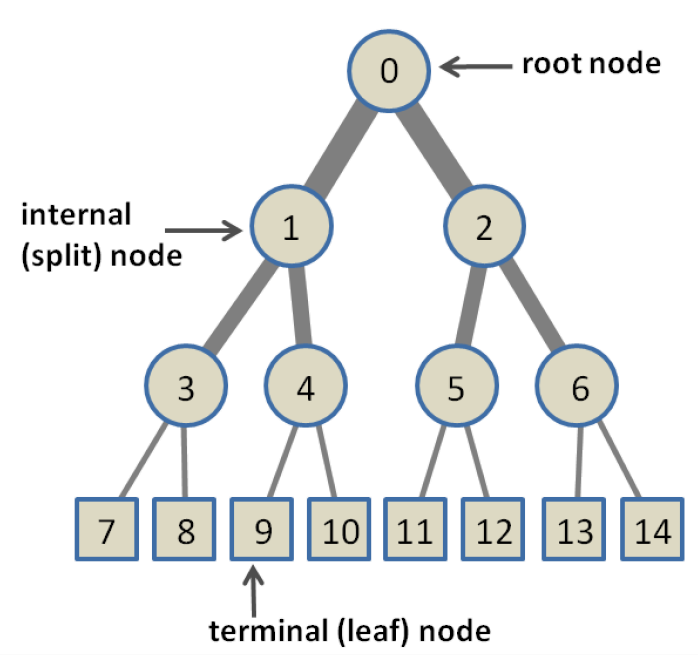
\includegraphics[width=0.35\textwidth]{images/DF}
	\caption{Schematically illustration example of a single decision tree}\label{f.df}
\end{figure}


The hyperparameters were determined by a individual grid search on the train date for the white matter, grey matter and cerebrospinal fluid. Visualized in Fig~(\ref{f.df_gridsearch}) are the results of the grid search for different number of nodes and trees, marked with a red cross. Unfortunately, it was not possible to achieve the best fit in every of three tissue types with the same hyperparameters. Therefore the chosen result of 160 trees and 3000 nodes was a trade off.

\begin{figure}[h!]
	\centering
	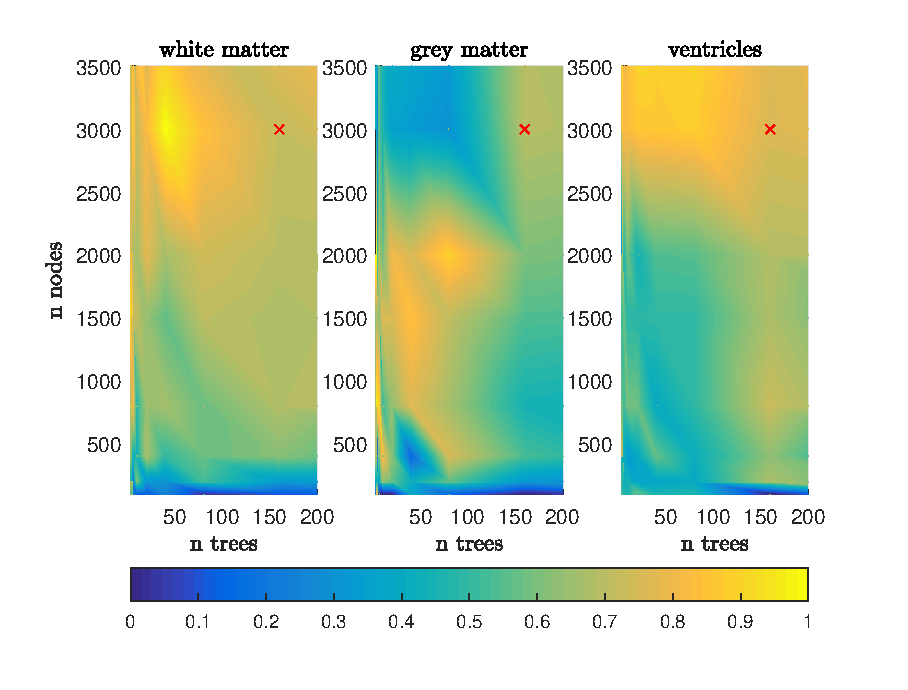
\includegraphics[width=0.48\textwidth]{images/df_grid}
	\caption{DF plot of grid search for white matter, grey matter and cerebrospinal fluid. The red cross marks the chosen hyperparameters number of trees~=~160 and maximum nodes per tree~=~3000. Color does not represent dice, the data is stretched individually for all three plots.}\label{f.df_gridsearch}
\end{figure}

\subsection{k-Nearest Neighbors (kNN)}
The k-Nearest Neighbors algorithm does not construct a general model, however stores instances of the training data. A query point is assigned to a certain class based on the votes, which come from the nearest neighbors of the point. A weight function assigns a weight which is inverse proportional to its distance to the point. The characteristics of kNN lead to a relatively low training time, and a rather high computation time for new points, depending on the amount of neighbors defined to vote. A hyperparameter search was conducted for the k-value. The higher k, the better the overall dice with the drawback of a higher computation time. A value of $k=20$ was found to be fast with only little trade-off in computation time.

\subsection{Support Vector Machine (SVM)}
Classification using Support Vector Machines (SVM) tries to find a hyperplane separating the data in a high-dimensional feature space. Given the feature vector $x_i$ and the binary label $y_i$, the SVM solves the following optimization problem during training:
\begin{equation}
\begin{split}
\min_{w, b, \xi} \ & \frac{1}{2}w^Tw + C\sum_{i=1}^m \xi_i \\
\ \text{ s.t. } & y_i(w^T\phi(x_i)+b) \geq 1-\xi_i, \; i = 1, \ldots, m \\
& \xi_i \geq 0, \; i = 1, \ldots, m
\end{split}
\end{equation}
where $w\in \mathbb{R}^n $ is the normal vector and $b \in \mathbb{R}$ the offset of the separating hyperplane and $\phi(x_i)$ maps $x_i$ into a higher-dimensional space.

The SVM implementation is based on libSVM \cite{chang2011libsvm}. Multiclass classification is solved with a \textit{one-against-one} approach. To output probabilities, the predictions are calibrated using \textit{Platt} scaling in which multiclass problems require an additional cross-validation which is an expensive operation for large datasets.

Given the relative low number of available features, we have chosen a radial basis function (RBF) kernel. A regularization term $C$ and a model capacity $\gamma$ needs to be chosen. These hyperparameters were determined with an exhaustive search and cross-validated on a subset of the training data, yielding $C=500$ and $\gamma=0.00005$.

\subsection{Stochastic Gradient Descent (SGD)}
Stochastic Gradient Descent (SGD) is widely used in machine learning for solving optimization problems iteratively. SGD has proven to be efficient for large-scale linear predictions \cite{zhang2004solving}.

In the current context, SGD learns a linear scoring function $f(x) = w^Tx + b$ with model parameters $w$ and $b$ by minimizing the training error
\begin{equation}
\argmin_{w,b} \frac{1}{m}\sum_{i=1}^mL(y_i, f(x_i)) + \alpha R(w)
\end{equation}
where $L$ is a loss function that measures miss-classifications, $R$ is a regularization term penalising model complexity, and $\alpha$ is a non-negative hyperparameter.

In each iteration, a sample is randomly chosen from the training set and the model parameters are updated according
\begin{equation}
w \leftarrow w - \eta \left(\alpha \frac{\partial R(w)}{\partial w} + \frac{\partial L (w^Tx_i + b, y_i)}{\partial w} \right)
\end{equation}
where $\eta$ is the learning rate controlling the step size.

We use a smoothed hinge loss (\textit{modified\_huber}) for the loss function $L$, a $l_2$ penalty ($||w||_2$) for the regularization term $R$, and a gradually decaying learning rate. This makes SGD similar to a linear SVM. Again, the hyperparameters $\eta = 0.5$ and $\alpha = 0.01$ were determined with an exhaustive search and cross-validated on a subset of the training data.


\subsection{Performance Evaluation}\label{ch.eval}
The Dice coefficient is a commonly used metric to compare the spatial overlap, ranging from 0 (no overlap) to 1 (perfect overlap). To evaluate the accuracy of the segmentation, a Dice coefficient is calculated between the prediction (E) and ground-truth (G) for each of the three labels. 
\begin{equation}
D = \frac{2|E \bigcap G|}{|E| + |G|} = \frac{2 TP}{2 TP + FP + FN}
\end{equation}

\section{Results}
\subsection{Segmentation Accuracy}
\begin{figure}
	\centering
	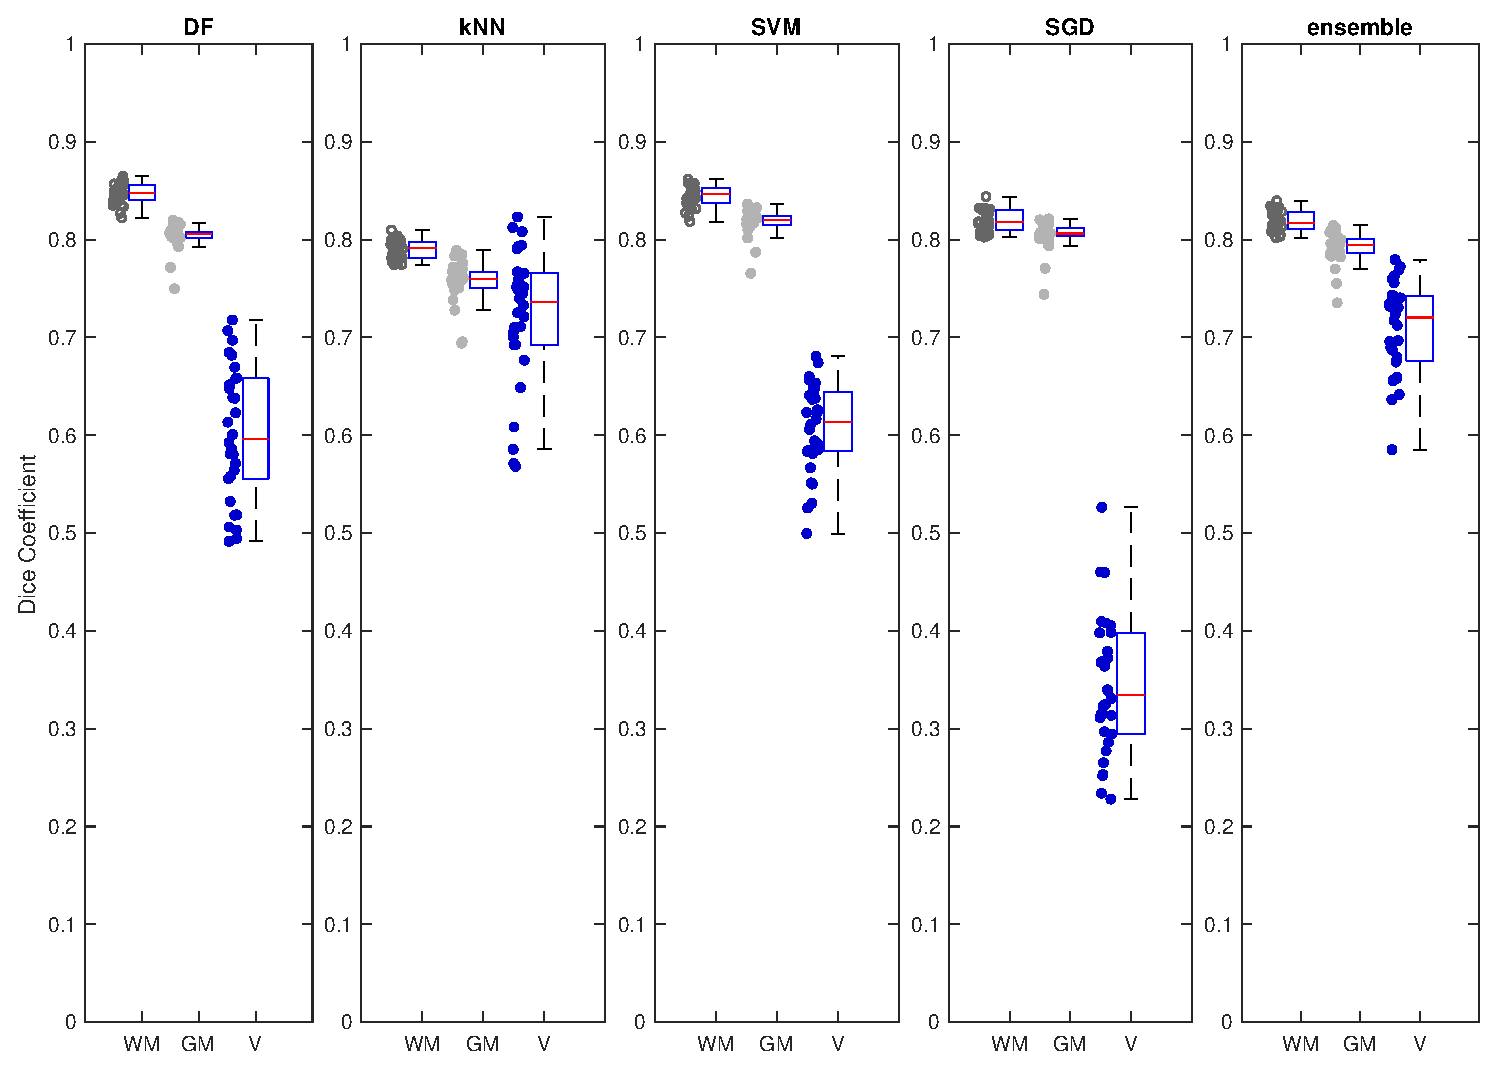
\includegraphics[width=0.48\textwidth]{images/boxplot}
	\caption{Distribution of dice coefficients with optimal hyper-parameters for each algorithm on the full training set of 70 images.}\label{f.boxplot}
\end{figure}

\begin{table*}[t]
\renewcommand{\arraystretch}{1.2}
\newcommand\mulrow[2]{\multirow{#1}{*}{\shortstack[c]{#2}}}
\caption{Performance Comparison of ML Algorithms}
\label{tab:perf_compare}
\centering
\begin{threeparttable}
\begin{tabular*}{0.9\textwidth}{@{\extracolsep{\fill}}c*{6}{S[table-number-alignment=center,table-figures-decimal=2,table-auto-round]}@{}}
\toprule
Features & {Size Dataset} & {\shortstack[c]{DF}} & {\shortstack[c]{kNN}} & {\shortstack[c]{SVM}} & {\shortstack[c]{SGD}} & {\shortstack[c]{ensemble}}\\
\midrule
\mulrow{3}{All\\(f1-f7)}
	& 3		&	{0.85/0.81/0.62} 	& {0.70/0.57/0.50}	& {0.83/0.80/0.61}	& {0.82/0.80/0.35}	& {-}\\
	& 12	&	{0.85/0.81/0.59}			& {0.75/0.66/0.67}	& {0.84/0.81/0.61}	& {0.82/0.80/0.34}	& {-}\\
	& 70	&	{0.85/0.80/0.60}			& {0.80/0.76/0.72}	& {0.84/0.82/0.61}	& {0.82/0.80/0.34}	& {0.82/0.79/0.71}\\
\midrule
\mulrow{3}{Coordinates only\\(f1-f3)}
	& 3		&	{0.67/0.63/0.22}		& {0.70/0.55/0.41}	& {0.59/0.52/0.0}	& {0.17/0.23/0.00}	& {-}\\
	& 12	&	{0.67/0.64/0.11}			& {0.74/0.63/0.56}	& {0.59/0.57/0.0}	& {0.19/0.22/0.00}	& {-}\\
	& 70	&	{0.67/0.64/0.16}			& {0.77/0.71/0.62}	& {0.60/0.58/0.31}	& {0.17/0.21/0.00}	& {-}\\
\midrule
\mulrow{3}{All non-coordinates \\(f4-f7)}
	& 3		&	{0.84/0.80/0.50}		& {0.85/0.80/0.45}	& {0.84/0.79/0.0}	& {0.82/0.80/0.34}	& {-}\\
	& 12	&	{0.85/0.80/0.49}			& {0.85/0.81/0.45}	& {0.85/0.80/0.45}	& {0.82/0.80/0.33}	& {-}\\
	& 70	&	{0.85/0.80/0.48}			& {0.85/0.81/0.54}	& {0.85/0.80/0.44}	& {0.82/0.80/0.34}	& {-}\\
\bottomrule
\end{tabular*}
\begin{tablenotes}
\item Overview of achieved accuracy for the different algorithms. Mean dice scores for white matter/grey matter/cerebrospinal fluid.
\item f1-f3: Coordinate features, f4: T1 intensity, f5: T1 gradient, f6: T2 intensity, f7: T2 gradient.
\end{tablenotes}
\end{threeparttable}
\end{table*}

All four optimized and examined algorithms are able to segment the MRI into the three tissue types. The performance measured by the dice coefficient for various configurations can be found in Tab.~(\ref{tab:perf_compare}). Boxplots with the statistical distributions for each algorithm on the whole test set and with all seven features can be seen in Fig. \ref{f.boxplot}.

The highest scores for combined WM and GM are reached by SVM with $0.84 \pm 0.01$ (WM) and $0.82 \pm 0.01$ (GM) but at the cost of a lower value for CSF ($0.61 \pm 0.05$). The highest mean value on CSF is reached by kNN with $0.72$ but also with the largest standard deviation of $\pm 0.07$ and lower mean values for WM ($0.80$) and GM ($0.76$). Although SGD is competitive on WM ($0.82 \pm 0.01$) and GM ($0.80 \pm 0.01$), the performance on CSF is the lowest ($0.34 \pm 0.07$).

The coordinate features seem to have a negative effect on the segmentation of WM and GM with kNN as this is the only algorithm reaching significant higher scores on those tissue types without using the coordinates, but with a negative effect on CSF.

The best dice coefficients are reached by combining the predictions from all algorithms to an ensemble.

\subsection{Training and Testing Time}
A comparison of the computation time both for training and testing is shown in Fig. \ref{f.runtimebarplot}.
\begin{figure}
	\centering
	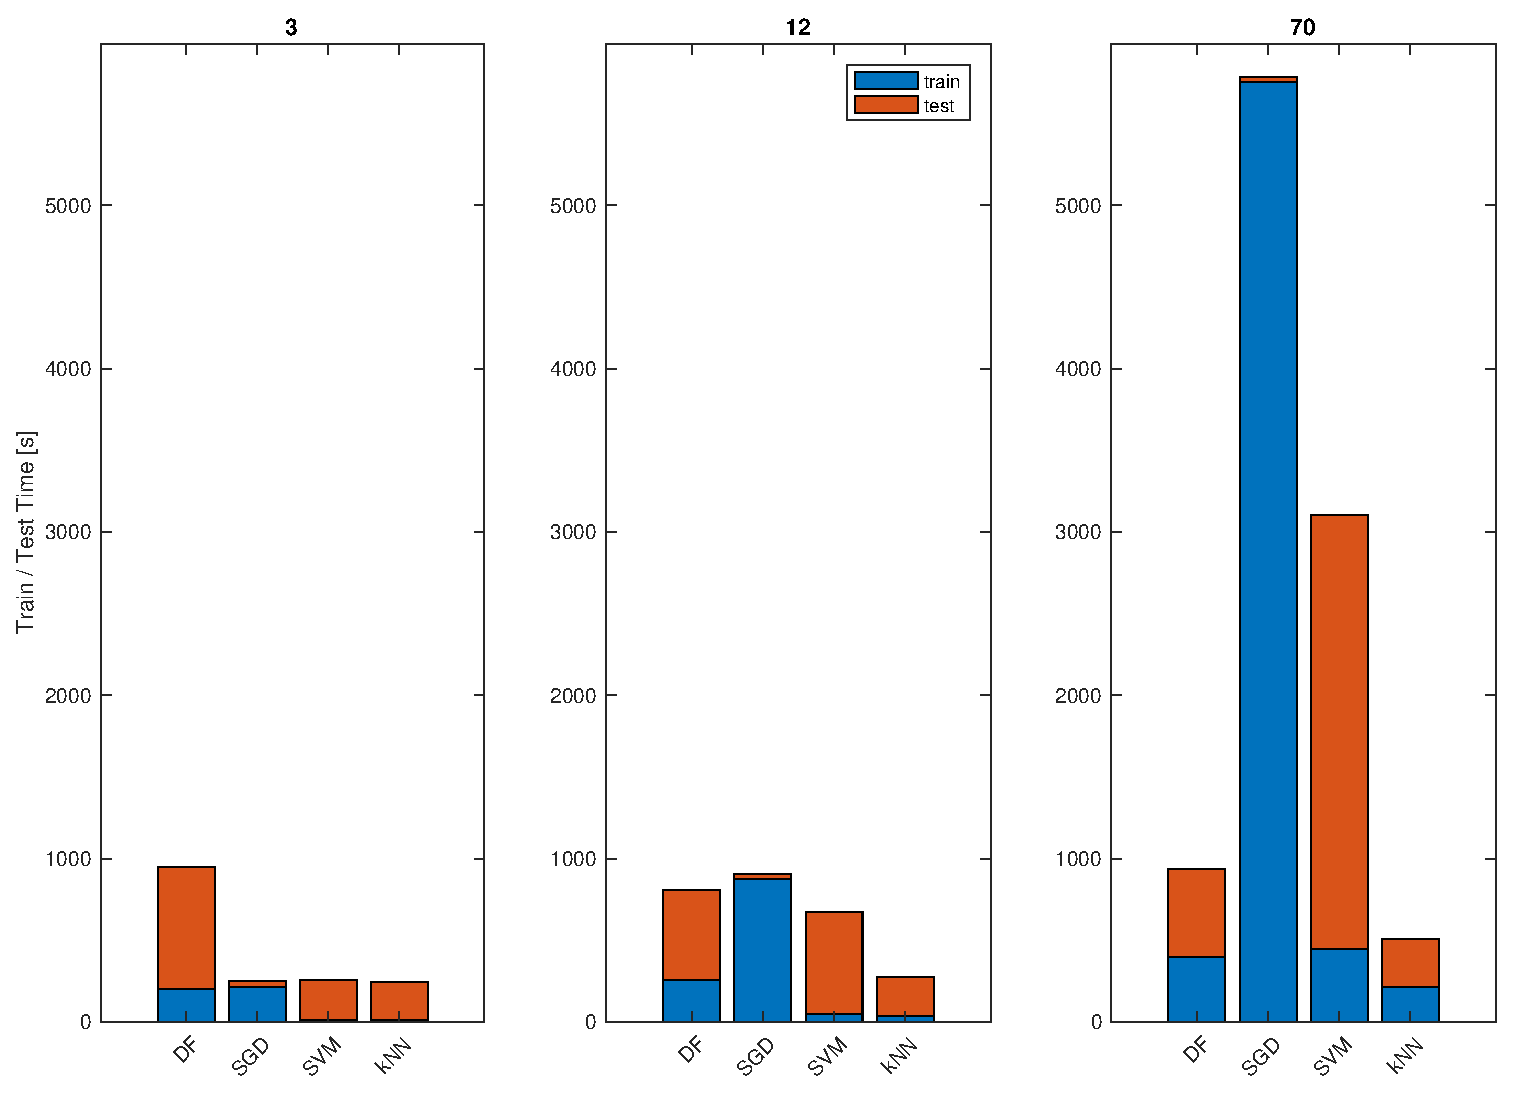
\includegraphics[width=0.48\textwidth]{images/runtimes}
	\caption{Time for training and testing of the algorithms with training set sizes of 3, 12 and 70 samples and using all seven features. Test time is for one sample and includes pre-processing, prediction and post-processing.}\label{f.runtimebarplot}
\end{figure}
Using the whole training set of 70 MR images, kNN is the fastest to train with $215s$, whereas SGD is the fastest on the prediction with only $42s$ per sample.

The training time is growing approximately linear with the amount of training data for kNN and SVM. For DF and SGD, the time required for training is growing significant slower than the amount of training data, leading to a good scaling behaviour.

For DF, kNN and SGD, the testing time is independent of the amount of training data used. Only for SVM the testing time is also growing with the size of the training data.

\subsection{Feature Inspection}

%Feature selection is another key part of the machine learning process. Features are also called variable or attribute and describe the model. Irrelevant and redundant features do not contribute to the accuracy of the predictive model, at worst they decrease the accuracy. The used feature set consists of seven features, f1-f3: Coordinate features, f4: T1 intensity, f5: T1 gradient, f6: T2 intensity, f7: T2 gradient. 

The following Fig~(\ref{scatterplot}) shows the scatter matrix of all the features. The whole dataset of 100 images was used for this evaluation. On the diagonal are the histograms to visualize the data distribution of each feature. The first three histograms are of the coordinate features and are normally distributed. The fifth and sixth histograms belong to the intensity features and follow a non normal distribution. The last two histograms are of the gradient features and are half normal distributed. The right upper part of the diagonal visualizes the linear correlation between each of the feature with the associated correlation coefficient. The left bottom part of the diagonal is redundant to the upper part. 

The coordinate features with an correlation coefficient between -0.12 and 0.05 are independent and do not correlate with any other feature at all. The first intensity feature has a moderate linear relationship with the second intensity feature and a weak with the first gradient feature. The second intensity feature has also a moderate correlation with both of gradient features. The gradient features correlate with an correlation coefficient of 0.83 very strong among themselves.


\begin{figure}[h]
	\centering
	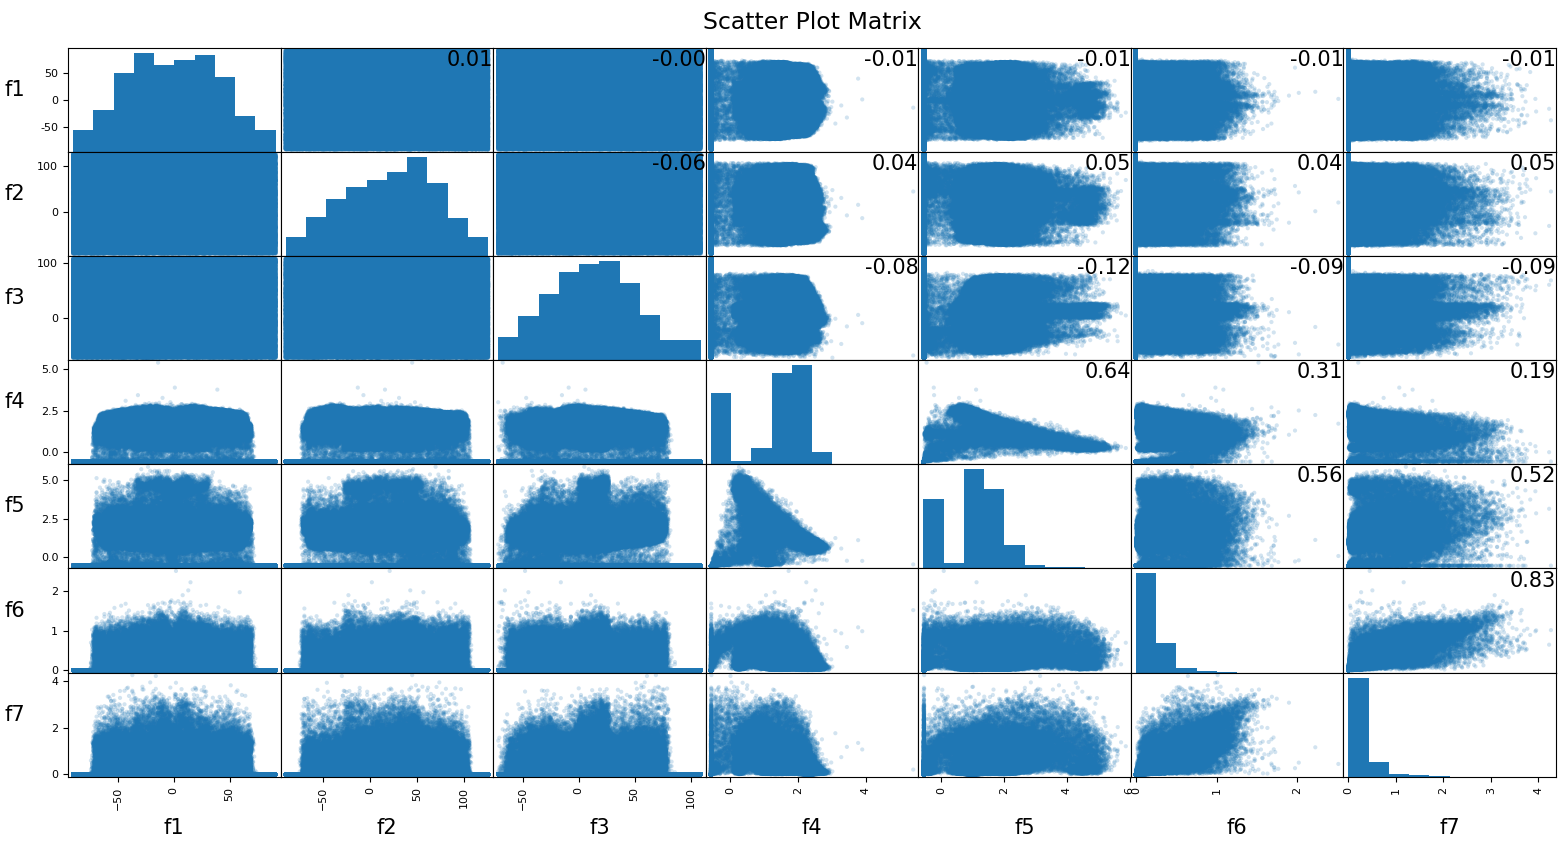
\includegraphics[width=0.48\textwidth]{images/ScatterPlotMatrix}
	\caption{Scatter plot of the features with associated correlation coefficient}
	\label{scatterplot}
\end{figure}

The following Fig~(\ref{FeatEval}) visualizes the influence of each feature type and the used algorithms. The feature types are divided in three coordinate, two intensity and two gradient features. The first column in this figure is calculated with all the features combined and is considered as a reference. Each column belongs to a single feature type in which the dice of the four used algorithms is visualized. Vertically in line is each dice for the gray matter, white matter and the cerebrospinal fluid disposed.

\TODO{Describe the plot, insert Legend of W, V or C? in figure 3, Mike, still waiting on one SVM}
\begin{figure}[h]
	\centering
	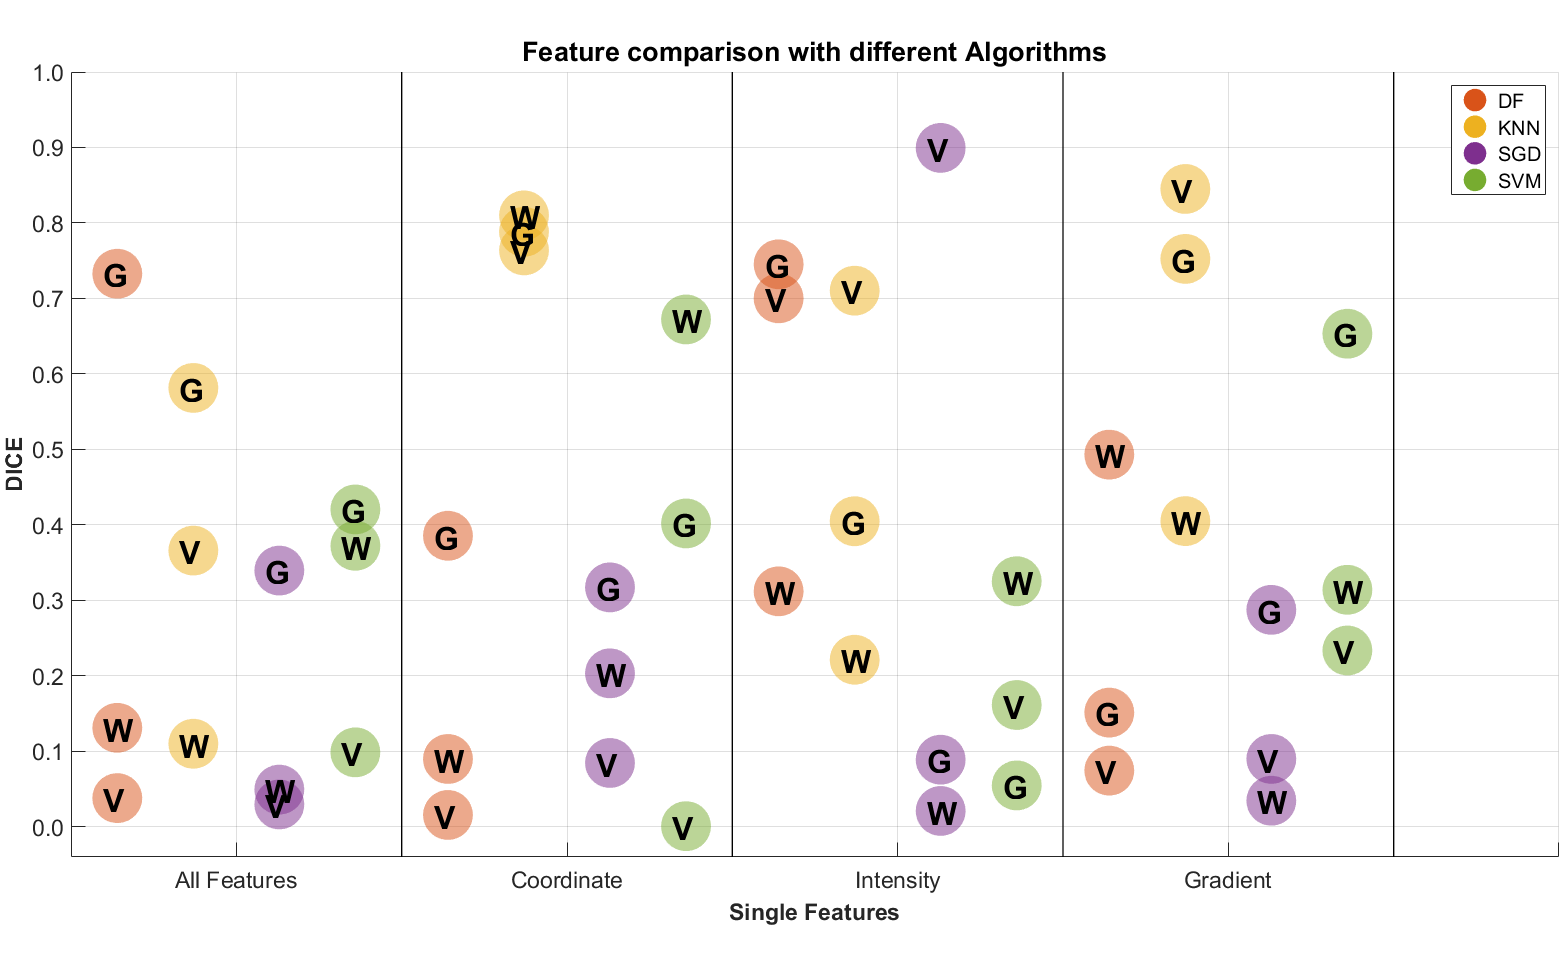
\includegraphics[width=0.49\textwidth]{images/FeatureEvaluation}
	\caption{Feature evaluation of single features with different algorithms, preprocessed.}
	\label{FeatEval}
\end{figure}




\subsection{Ground Truth Validity}

A sample of a ground truth segmentation can be seen in Fig.~\ref{f.slice_ground_truth}. By comparing this image with the other images in Fig.~\ref{f.slices_all} it is obvious that there is some misclassification in the ground truth figure. Especially the center of the brain is mainly classified as background, which is undeniably wrong. Furthermore, there is no matter classified as CSF outside of the GM, although it is anatomically incorrect. The algorithms presented in this work depend, among other features (see Sec.~\ref{s.pipeline}) on the coordinates of the voxels. Therefore, there are barely any CSF classifications outside of the GM made by the tested algorithms as well.



\subsection{Random Mask Optimization}

Tuning the random mask (see Sec.~\ref{s.pipeline}) turned out to be crucial to improve the classification of CSF. A first approach to take approximately the same absolute numbers from all voxel types turned out to be suboptimal. Better results were achieved by including roughly the same proportion of voxels from WM, GM and CSF. From the background class however, which has the highest absolute number of voxels, approximately the same number of voxels as from the other classes were taken. The fraction of voxels taken into account are therefore 0.004 for WM and CSF, 0.003 for GM, and 0.0003 for background. Except for SGD where a better segmentation is achieved with 0.04 for CSF which results in approximately the same amount of voxels from all types to be used for training.

\begin{figure}[h!]
	\centering
	\subfloat[DF]{\label{f.slice_df}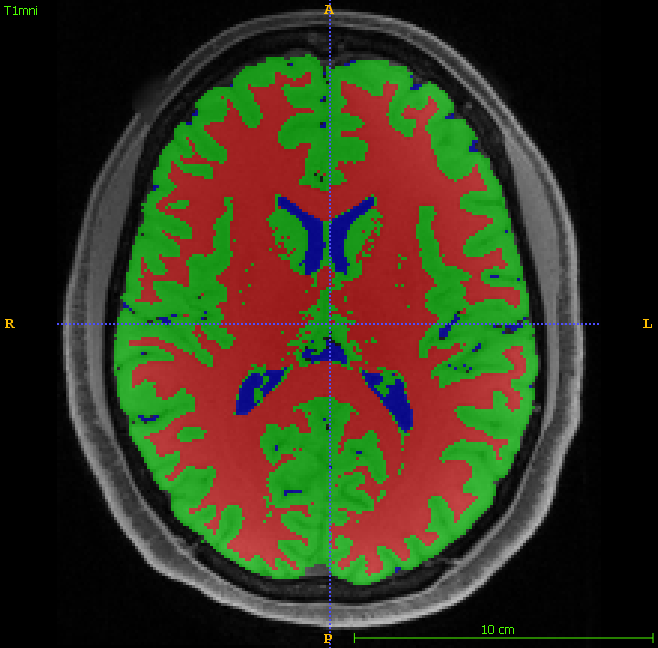
\includegraphics[width=0.3\linewidth]{images/slice_DF}}
	\hfill
	\subfloat[kNN]{\label{f.slice_knn}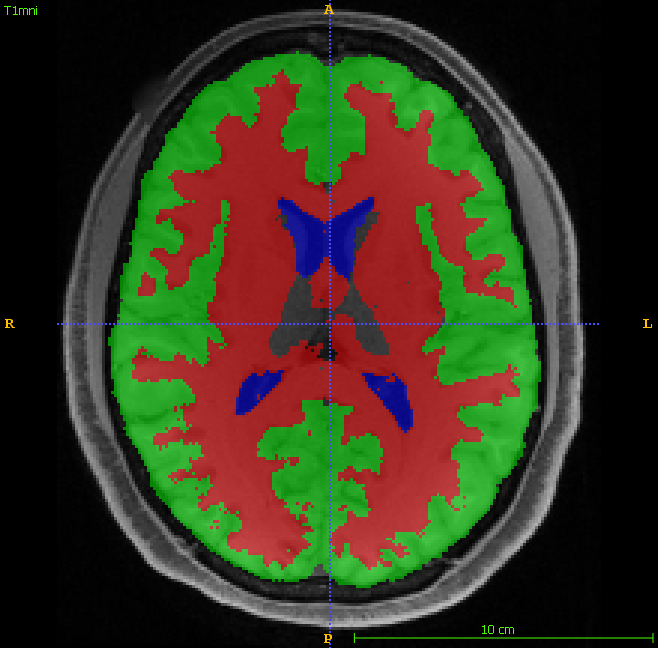
\includegraphics[width=0.3\linewidth]{images/slice_kNN}}
	\hfill
	\subfloat[SVM]{\label{f.slice_svm}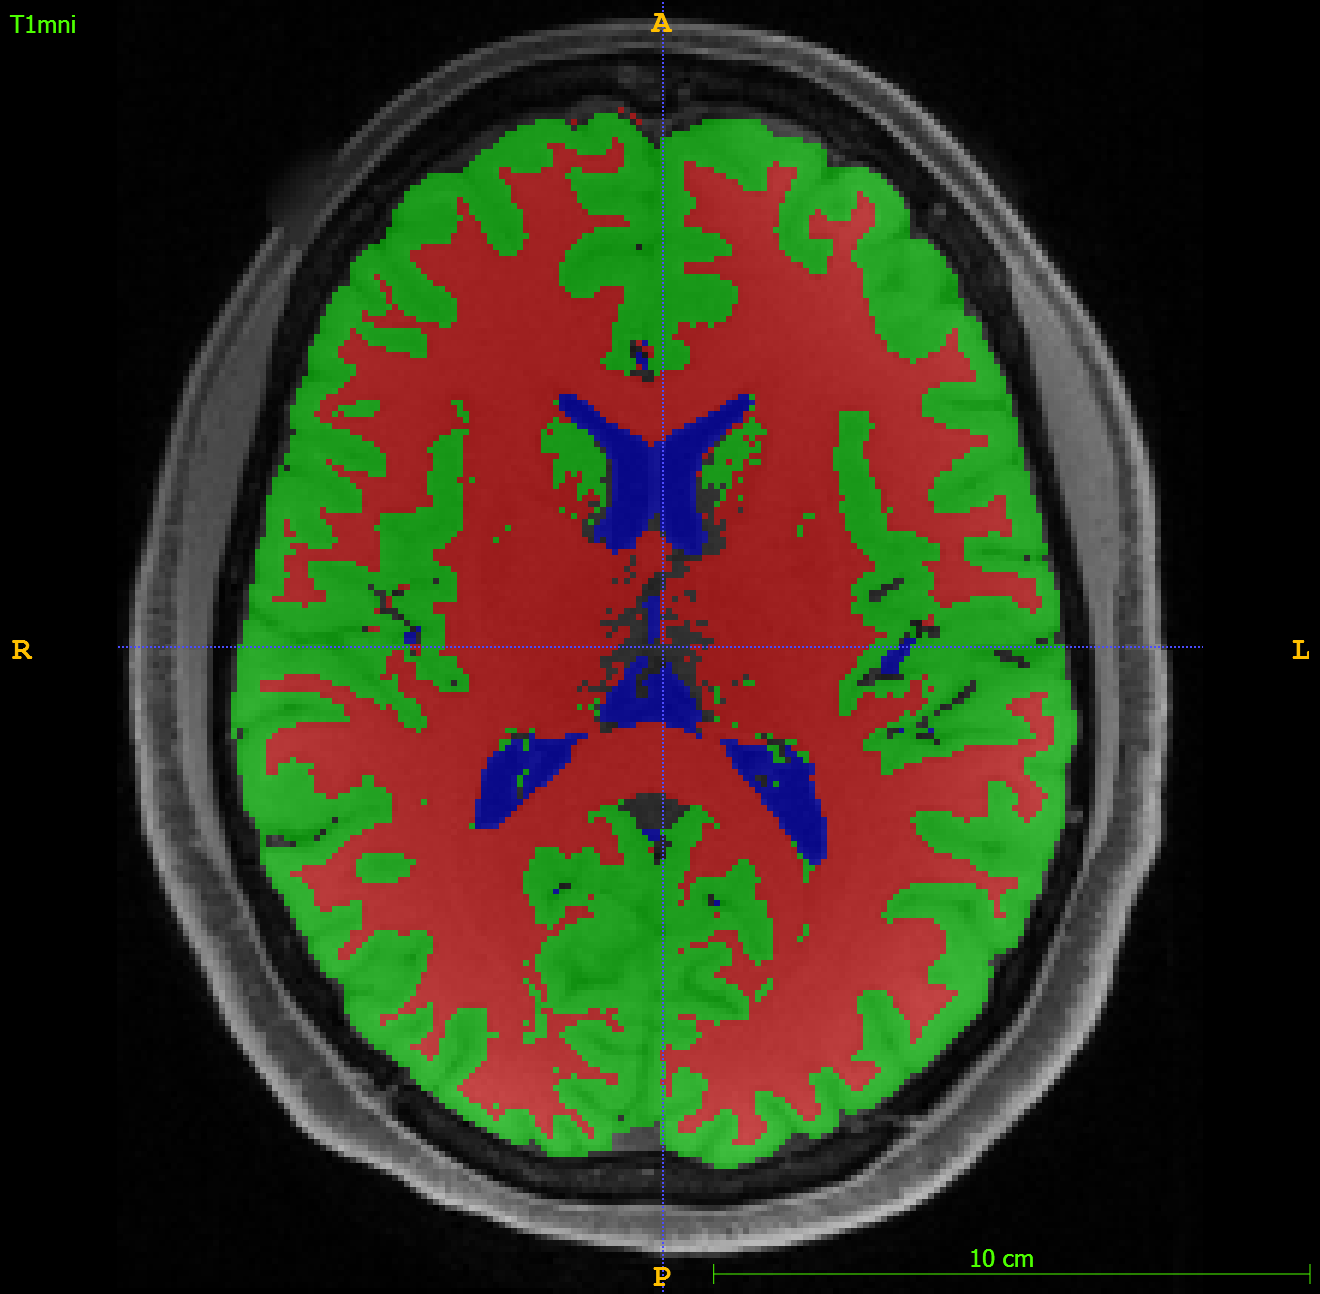
\includegraphics[width=0.3\linewidth]{images/slice_SVM}}
	\hfill
	\subfloat[SGD]{\label{f.slice_sgd}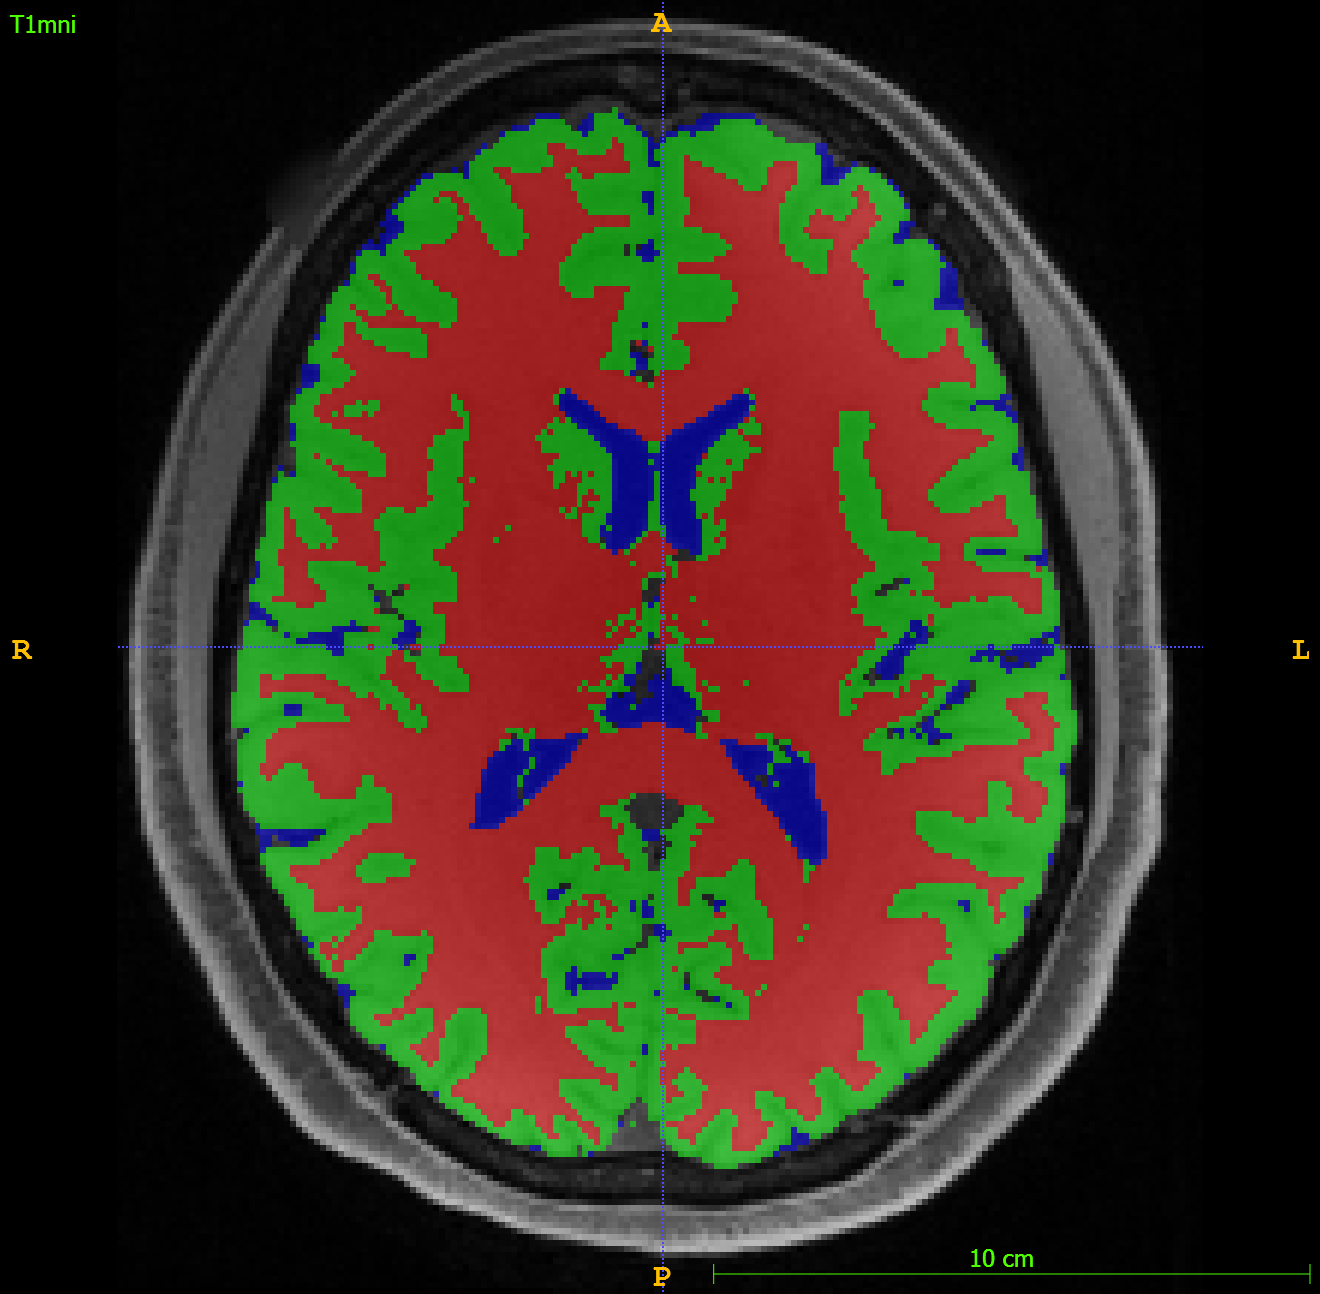
\includegraphics[width=0.3\linewidth]{images/slice_SGD}}
	\hfill
	\subfloat[ensemble]{\label{f.slice_ensemble}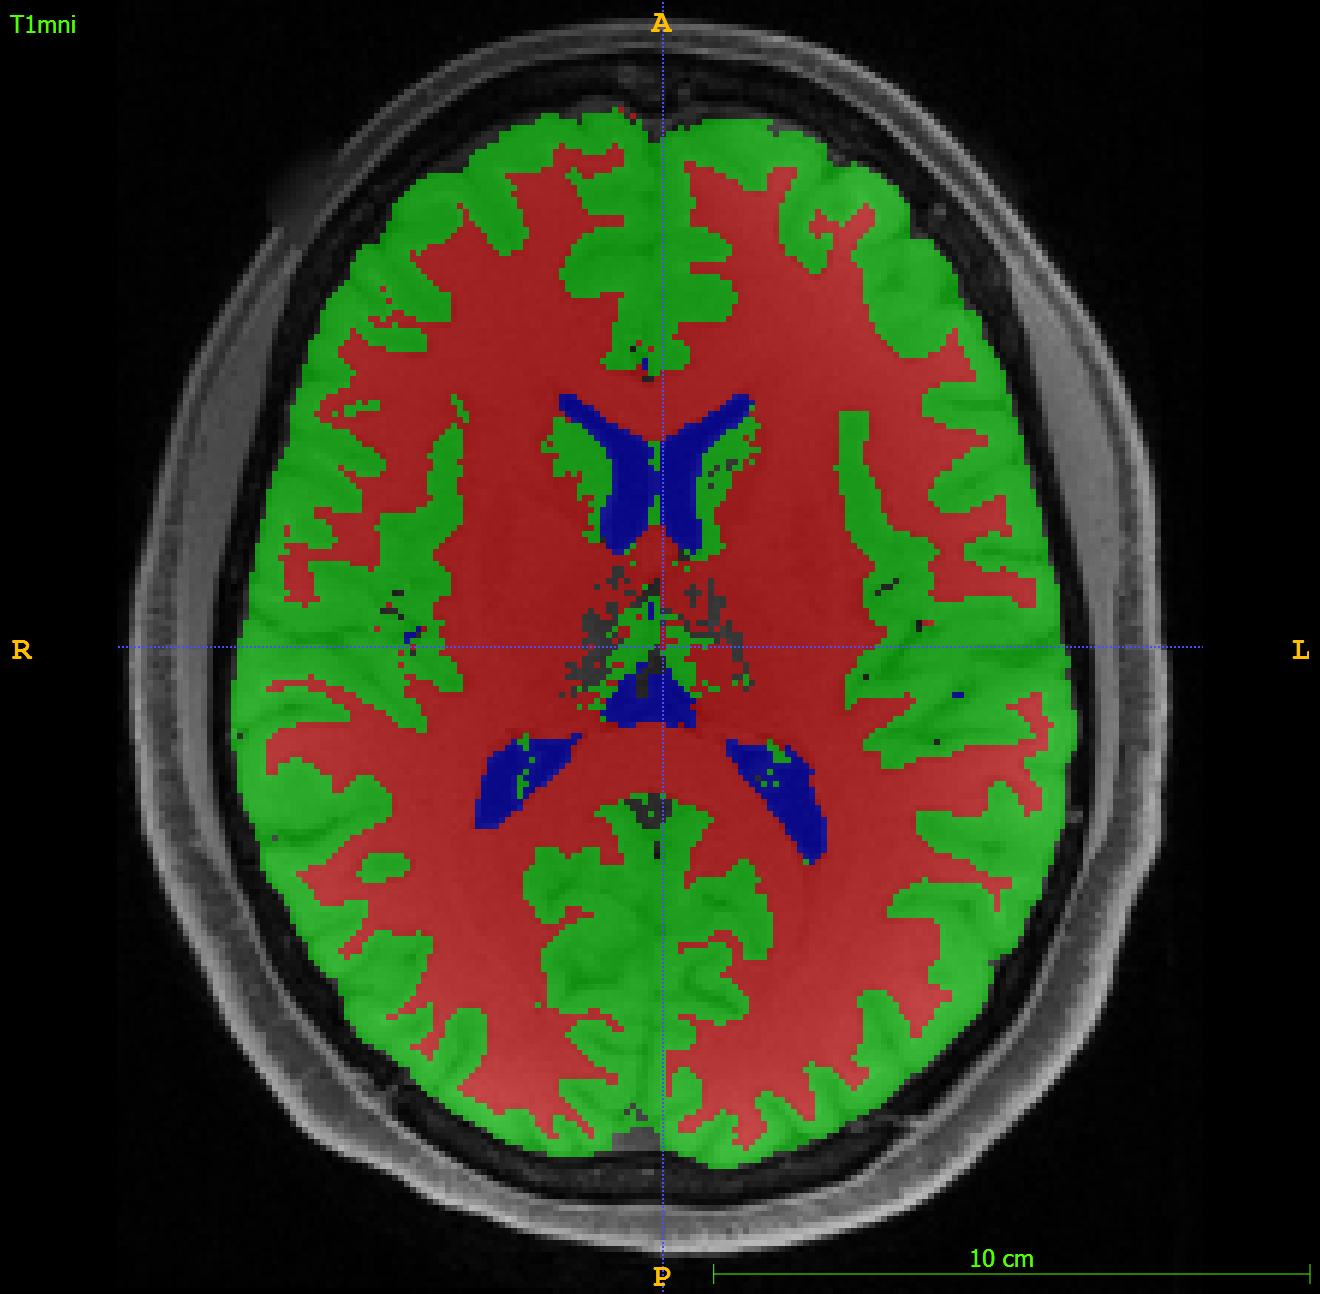
\includegraphics[width=0.3\linewidth]{images/slice_ensemble}}
	\hfill
	\subfloat[ground truth]{\label{f.slice_ground_truth}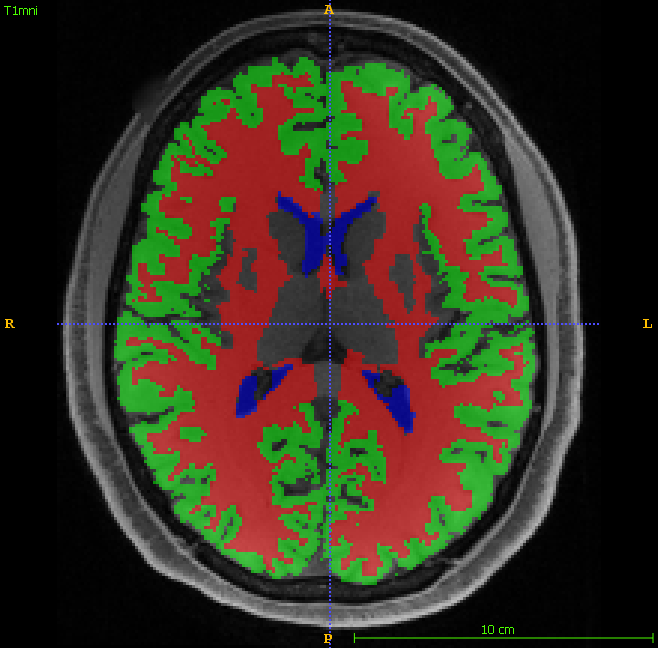
\includegraphics[width=0.3\linewidth]{images/slice_ground_truth}}
	%\caption{Slices of best performances of \protect\subref{f.slice_df} DF, \protect\subref{f.slice_knn} kNN, \protect\subref{f.slice_svm} SVM, \protect\subref{f.slice_sgd} SGD, \protect\subref{f.slice_ensemble} ensemble, and \protect\subref{f.slice_ground_truth} ground truth.}
	\caption{Segmentation of optimal tuned algorithms, ensemble, and ground truth. All images are from the same head, on the same slice. }
	\label{f.slices_all}
\end{figure}

\section{Discussion}
With our experiments, we could confirm DF is a good default choice for the segmentation of brain tissue in MRI data. All four examined algorithms reach a similar accuracy but with different runtime behaviour. DF and SGD allow for an incremental training where input data can be processed sequentially in batches of arbitrary sizes. kNN and SVM on the other hand require all training data to be hold in memory, which inherently limits their application. Large amounts of data are trained most efficiently with SGD, few data with SVM. This observation is consistent with the mathematical foundation of these two algorithms. The good scaling behaviour of stochastic gradient descent is based on the principle of approximating a gradient by randomly (stochastically) choosing samples out of a large dataset and not necessary having to consult all data points in each iteration. A support vector machine might find a solution with a limited number of samples by mapping low dimensional features to a higher dimensional feature space where the data is more likely to be separable. Although this comes with high computational costs for fitting such a complex model to a larger amount of data.

We have observed a rather small influence of the size of the training set, DF, SVM, and SGD reaching a similar dice coefficient with either 3 or 70 training samples. This might be due to the limited number of features used. With additional features, the amount of training data might become more important.

The segmentation of CSF yielded the lowest dice coefficients across all algorithms. We partially attribute this to the ground truth data which is of equivocal quality especially in the CSF regions. A manual augmentation of the data by experts is required to judge how much is indeed related to this.

The dataset includes only MRI from healthy individuals. How well the segmentation generalizes for anatomical disturbances, tumors or brain diseases remains to be tested.

Finally, we have only combined the algorithms to a simple ensemble by taking the max. probability for each voxel from the predictions. Advanced combinations like sequentially applying two methods or use one method on a global level and the other on a local level might further improve the results.

\section{Conclusion}
The major challenge remains the quality of ground-truth data. As long as the test set is the output from an other (imperfect) algorithm, any approach is just an approximation of the other mechanism.

In the current setup, the number of available features was limited to seven which is known to be on the lower bound for the examined algorithms. A deep learning approach that is directly processing the raw input data and implicitly learning how to extract features might be a better choice in this case. Whether such a neural network outperforms the classical machine learning algorithms remains to be investigated.

\section*{Acknowledgement}
Calculations were performed on UBELIX (http://www.id.unibe.ch/hpc), the HPC cluster at the University of Bern.

\bibliographystyle{IEEEtran}
\bibliography{references}

\end{document}